\documentclass[a4paper,11pt,titlepage]{article}
\usepackage[czech]{babel}
\usepackage[utf8]{inputenc}
\usepackage{rotating}
\usepackage{graphicx}
\pagestyle{headings}
\author{Radka Mokrá, Lukáš Brabec, Aleš Dujíček, Jan Sedlák}
\title{Dokumentace k projektu pro předměty IAL a IFJ}
\frenchspacing

\begin{document}
%\maketitle
\thispagestyle{empty}

\begin{center}
\Large{\scshape Vysoké učení technické v Brně}

\vspace{0.5cm}

\large{Fakulta informačních technologií}

\vfill

\Large{\scshape Dokumentace k projektu pro přeměty IAL a IFJ}

% \vspace{0.5cm}
%
% 2010/2011

\vfill

\LARGE{Překladač jazyka IFJ11}

\vfill

\large{Tým 097, varianta a/1/I}
\end{center}

\vspace{0.5cm}

\begin{tabular}{l l r l}
Radka Mokrá  & \tt{xmokra00} & 34\% & vedoucí \\ 
Lukáš Brabec & \tt{xbrabe09} &  0\% & \\
Aleš Dujíček & \tt{xdujic01} & 33\% & \\
Jan Sedlák   & \tt{xsedla85} & 33\% & \\
\end{tabular}

%\begin{flushright}
%\today
%\end{flushright}

\newpage{}


\tableofcontents

\newpage

\section{Úvod}
Tento text je dokumentací k týmovému projektu do kurzu IFJ (Formální jazyky a překladače) a IAL (Algoritmy). Popisuje implementaci interpretru jazyka inspirovaného programovacím jazykem Lua. Pro řešení byla vybrána varianta a/1/I, řazení je implementováno algoritmem quicksort, tabulka symbolů binárním stromem a vyhledávání podřetězců Knuth-Morris-Prat\-to\-vým algoritmem.

\section{Lexikální analýza}
Lexikální analyzátor je navržen a implementován jako deterministický ko\-neč\-ný automat, jehož graf přechodů je zobrazen na obrázku \ref{lex.lex}. Symbol \ae{} značí všechny ostatní symboly, pro které z daného stavu není jiný přechod.

\begin{figure}[h!]
\centering
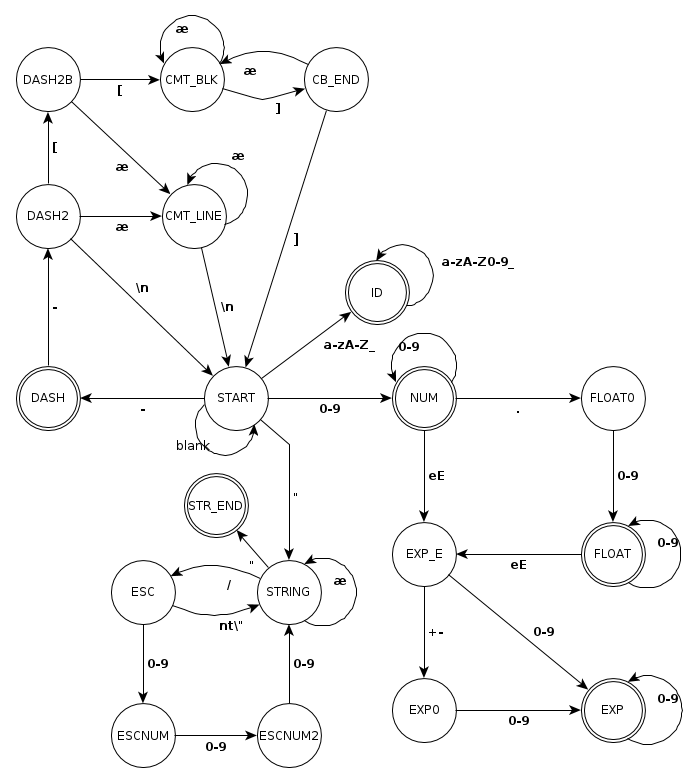
\includegraphics[width=11cm]{lexical.png}
\caption{Schéma konečného automatu lexikálního analyzátoru}
\label{lex.lex}
\end{figure}

V koncovém stavu pro indentifikátory skončí i klíčová a rezervovaná slova. Kdyby je měl automat zpracovávat zvlášť, přibylo by mnoho stavů a automat by se stal nepřehledným. Proto jsou zpracovány spolčně s identifikátory a na konci je volána funkce, která určí, zda se skutečně jedná o identifikátor, nebo některé z klíčových nebo rezervovaných slov.

Graf na obázku \ref{lex.lex} není úplný, zobrazuje jen analýzu řetězců, identifikátorů, čísel a komentářů. Analýza ostatních lexémů, jedná so o operátory, je realizována jen jedním, případně dvěma, přechody z počátečního stavu {\tt start}. Graf by se ale při takovém množství přechodů z počátečního stavu stal nepřehledným. Proto je jejich zpracování zobrazeno obrázku \ref{lex.ope} zvlášť od složitější a zajímavější části automatu.

\begin{figure}
\centering
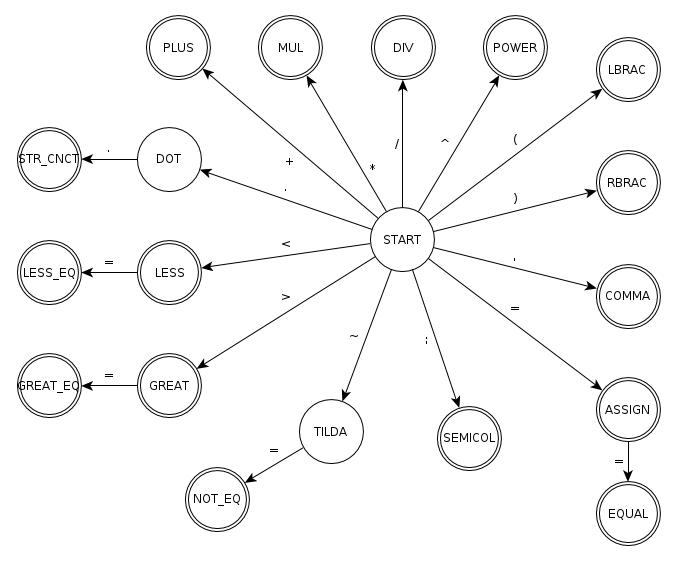
\includegraphics[width=10cm]{operator.png}
\caption{Schéma konečného automatu lexikálního analyzátoru}
\label{lex.ope}
\end{figure}


\section{Syntaktická analýza}
program $ \rightarrow $ definice-funkce   definice-funkcí   \textbf{;}   \textbf{EOF} \\
definice-funkce $ \rightarrow $	\textbf{function} \textbf{id} \textbf{(} parametry \textbf{)} deklarace příkazy \textbf{end} \\
definice-funkcí $ \rightarrow $ definice-funkce   definice-funkcí \\
definice-funkcí $ \rightarrow \varepsilon $ \\
parametry $ \rightarrow $	\textbf{identifier}   parametry-z \\
parametry $ \rightarrow \varepsilon $ \\
parametry-z $ \rightarrow $ \textbf{,}   \textbf{id} parametry-z \\
parametry-z $ \rightarrow 	\varepsilon $ \\
deklarace $ \rightarrow $	\textbf{local} \textbf{id} deklarace-z   deklarace \\
deklarace $ \rightarrow \varepsilon $ \\
deklarace-z $ \rightarrow $ \textbf{=} výraz \textbf{;} \\
deklarace-z $ \rightarrow $ \textbf{;} \\
literál $ \rightarrow $	\textbf{číslo} \\
literál $ \rightarrow $ \textbf{řetězec} \\
literál $ \rightarrow $ \textbf{nil} \\
literál $ \rightarrow $ \textbf{true} \\
literál $ \rightarrow $ \textbf{false} \\ 
sekvence-příkazů $ \rightarrow $	příkaz   \textbf{;}   sekvence-příkazů \\
sekvence-příkazů $ \rightarrow \varepsilon $ \\
příkaz $ \rightarrow $	\textbf{id} \textbf{=} assign-z \\
příkaz $ \rightarrow $	\textbf{write} \textbf{(} seznam-výrazů \textbf{)} \\
příkaz $ \rightarrow $	\textbf{if} výraz \textbf{then} sekvence-příkazů \textbf{else} sekvence-příkazů \textbf{end} \\
příkaz $ \rightarrow $	\textbf{while} výraz \textbf{do} sekvence-příkazů \textbf{end} \\
příkaz $ \rightarrow $	\textbf{return} výraz \\
příkaz $ \rightarrow $	\textbf{repeat} sekvence-příkazů \textbf{until} výraz \\
assign-z $ \rightarrow $ \textbf{read}   \textbf{(}  literál \textbf{)} \\
assign-z $ \rightarrow $ výraz \\
seznam-výrazů $ \rightarrow $ výraz seznam-výrazů-z \\
seznam-výrazů-z $ \rightarrow $ \textbf{,} výraz seznam-výrazů-z \\
seznam-výrazů-z $ \rightarrow \varepsilon $ \\


\subsection{Analýza výrazů}
Analýza výrazů je obstrána funkcí {\tt expression()}, kterou zavolá parser, když je dle pravidel očekáván výraz. Výrazy jsou zpracovány pomocí precedenční syntaktické analýzy zdola nahoru. Pro tuto potřebu byla vytvořena precedenční tabulka, ktérá určuje pořadí, v jakém jsou vyhodnoceny jedntlivé části výrazu. 
\begin{sidewaystable}
\centering
\begin{tabular}{l | c c c c c c c c c c c c c c c c c c c c c}
      & \^{} & * & / & + & - & ..& $<$ & $>$ & $<$= & $>$= & ~= & == & id & num & str & bool & nil & (  & )  & ,  & \$ \\ \hline
  \^{}  & $<$ & $>$ & $>$ & $>$ & $>$ & $>$ & $>$ & $>$ & $>$  & $>$  & $>$  & $>$  & $<$  & $<$   & $<$   & $<$    &  $<$  & $<$  & $>$  & $>$  & $>$ \\
  *     & $<$ & $>$ & $>$ & $>$ & $>$ & $>$ & $>$ & $>$ & $>$  & $>$  & $>$  & $>$  & $<$  & $<$   & $<$   & $<$    &  $<$  & $<$  & $>$  & $>$  & $>$ \\
  /     & $<$ & $>$ & $>$ & $>$ & $>$ & $>$ & $>$ & $>$ & $>$  & $>$  & $>$  & $>$  & $<$  & $<$   & $<$   & $<$    &  $<$  & $<$  & $>$  & $>$  & $>$ \\
  +     & $<$ & $<$ & $<$ & $>$ & $>$ & $>$ & $>$ & $>$ & $>$  & $>$  & $>$  & $>$  & $<$  & $<$   & $<$   & $<$    &  $<$  & $<$  & $>$  & $>$  & $>$ \\
  -     & $<$ & $<$ & $<$ & $>$ & $>$ & $>$ & $>$ & $>$ & $>$  & $>$  & $>$  & $>$  & $<$  & $<$   & $<$   & $<$    &  $<$  & $<$  & $>$  & $>$  & $>$ \\
  ..    & $<$ & $<$ & $<$ & $<$ & $<$ & $>$ & $>$ & $>$ & $>$  & $>$  & $>$  & $>$  & $<$  & $<$   & $<$   & $<$    &  $<$  & $<$  & $>$  & $>$  & $>$ \\
  $<$     & $<$ & $<$ & $<$ & $<$ & $<$ & $<$ & $>$ & $>$ & $>$  & $>$  & $>$  & $>$  & $<$  & $<$   & $<$   & $<$    &  $<$  & $<$  & $>$  & $>$  & $>$ \\
  $>$     & $<$ & $<$ & $<$ & $<$ & $<$ & $<$ & $>$ & $>$ & $>$  & $>$  & $>$  & $>$  & $<$  & $<$   & $<$   & $<$    &  $<$  & $<$  & $>$  & $>$  & $>$ \\
  $<$=    & $<$ & $<$ & $<$ & $<$ & $<$ & $<$ & $>$ & $>$ & $>$  & $>$  & $>$  & $>$  & $<$  & $<$   & $<$   & $<$    &  $<$  & $<$  & $>$  & $>$  & $>$ \\
  $>$=    & $<$ & $<$ & $<$ & $<$ & $<$ & $<$ & $>$ & $>$ & $>$  & $>$  & $>$  & $>$  & $<$  & $<$   & $<$   & $<$    &  $<$  & $<$  & $>$  & $>$  & $>$ \\
  ~=    & $<$ & $<$ & $<$ & $<$ & $<$ & $<$ & $>$ & $>$ & $>$  & $>$  & $>$  & $>$  & $<$  & $<$   & $<$   & $<$    &  $<$  & $<$  & $>$  & $>$  & $>$ \\
  ==    & $<$ & $<$ & $<$ & $<$ & $<$ & $<$ & $>$ & $>$ & $>$  & $>$  & $>$  & $>$  & $<$  & $<$   & $<$   & $<$    &  $<$  & $<$  & $>$  & $>$  & $>$ \\
  id    & $>$ & $>$ & $>$ & $>$ & $>$ & $>$ & $>$ & $>$ & $>$  & $>$  & $>$  & $>$  &    &     &     &      &     & =  & $>$  & $>$  & $>$ \\
  num   & $>$ & $>$ & $>$ & $>$ & $>$ & $>$ & $>$ & $>$ & $>$  & $>$  & $>$  & $>$  &    &     &     &      &     &    & $>$  & $>$  & $>$ \\
  str   & $>$ & $>$ & $>$ & $>$ & $>$ & $>$ & $>$ & $>$ & $>$  & $>$  & $>$  & $>$  &    &     &     &      &     &    & $>$  & $>$  & $>$ \\
  bool  & $>$ & $>$ & $>$ & $>$ & $>$ & $>$ & $>$ & $>$ & $>$  & $>$  & $>$  & $>$  &    &     &     &      &     &    & $>$  & $>$  & $>$ \\
  nil   & $>$ & $>$ & $>$ & $>$ & $>$ & $>$ & $>$ & $>$ & $>$  & $>$  & $>$  & $>$  &    &     &     &      &     &    & $>$  & $>$  & $>$ \\
  (     & $<$ & $<$ & $<$ & $<$ & $<$ & $<$ & $<$ & $<$ & $<$  & $<$  & $<$  & $<$  & $<$  & $<$   & $<$   & $<$    &  $<$  & $<$  & =  & $<$  &   \\
  )     & $>$ & $>$ & $>$ & $>$ & $>$ & $>$ & $>$ & $>$ & $>$  & $>$  & $>$  & $>$  &    &     &     &      &     &    & $>$  & $>$  & $>$ \\
  ,     & $<$ & $<$ & $<$ & $<$ & $<$ & $<$ & $<$ & $<$ & $<$  & $<$  & $<$  & $<$  & $<$  & $<$   & $<$   & $<$    &  $<$  & $<$  & $>$  & $>$  & $>$ \\
  \$    & $<$ & $<$ & $<$ & $<$ & $<$ & $<$ & $<$ & $<$ & $<$  & $<$  & $<$  & $<$  & $<$  & $<$   & $<$   & $<$    &  $<$  & $<$  &    & $<$  &   \\
\end{tabular}
\caption{Precenenční tabulka syntaktické analýzy výrazů}
\label{tab.prec}
\end{sidewaystable} 

Výrazy jsou tvořeny literály, již definovanými proměnnými, závorkami nebo výrazy tvořenými binárními aritmetickými a relačními o\-pe\-rá\-to\-ry. Na rozdíl od jazyka Lua nejsou implicitní konverze povoleny až na specifikované výjimky. Případy, kdy je operand dané operace nekompatibilního typu, se dělí na dvě možnosti. Pokud je operand literál, je o chybě rozhodnouto již v době analýzy zdrojového kódu a jedná se o sémantickou chybu. V případě, že operand není literál, jedná se o chybu interpretace. 
Volání funkcí je zpracováno jako výraz a funkce mohou být součástí výrazu, zároveň mohou být výrazy v parametrech funkcí.

\begin{figure}
$ E \rightarrow id $ \\
$ E \rightarrow	lit $ \\
$ E \rightarrow E $ \^{ } $ E $ \\
$ E \rightarrow	E * E $ \\
$ E \rightarrow	E / E $ \\
$ E \rightarrow E + E $ \\
$ E \rightarrow	E - E $ \\
$ E \rightarrow	E .. E $ \\
$ E \rightarrow	E < E $ \\
$ E \rightarrow	E > E $ \\
$ E \rightarrow	E <= E $ \\
$ E \rightarrow	E >= E $ \\
$ E \rightarrow	E ~= E $ \\
$ E \rightarrow	E == E $ \\
$ E \rightarrow	( E ) $ \\
$ E \rightarrow	id ( E ) $ \\
$ E \rightarrow	id ( P ) $ \\
$ P \rightarrow E, E $ \\
$ P \rightarrow	P, E $ \\
\caption{Pravidla gramatiky výrazů}
\label{syn.expr}
\end{figure}


\section{Sémantická analýza}

\section{Interpretace}

Pro účely našeho interpreteru používáme variantu tříadresného kódu. Pro\-to\-že veškeré aritmetické a porovnávací instrukce pracují se zásobníkem, je v instrukcích potřeba maximálně jediná adresa.

\subsection{Zásobník}

V našem interpreteru hraje zásobník důležitou roli. Používá se jak pro lokální proměnné a předávání argumentů funkcím tak pro veškeré výpočty. Jelikož parser pro výrazy dokáže výraz jednoduše převést do postfixové formy, rozhodli jsme se, že instrukce ADD, SUB apod. budou pracovat s čísly, které jsou uloženy na zásobníku. Například kód {\tt a = 3 + 4} se převede do instrukcí {\tt push 4; push 3; add; popi a}. Toto sice není nejlepší řešení z pohledu rychlosti interpretace a optimalizací, za to je velice snadný pro implementaci. Pro implementaci zásobníku používáme dynamicky alokované (a realokovatelné) pole. Používáme také \uv{registry} ESP, EBP a EIP po řadě pro ukazatel na vrchol zásobníku, ukazatel pro přístup k lokálním proměnným a ukazatel na aktuálně prováděnou instrukci.

\subsection{Páska instrukcí}

Páska instrukcí je implementována pomocí zřetězeného lineárního jedno\-směr\-né\-ho seznamu, jelikož není potřeba se mezi instrukcemi posouvat zpět (a při skocích je známa adresa, na kterou instrukci musí interpret skočit). Vhodně se také dá využít aktuální prvek seznamu (jako příznak pro instrukci, která bude aktuálně prováděná).

\subsection{Volání funkcí a návrat z funkce}

Pro volání funkcí jsme se inspirovali u assembleru pro platformu x86 a volání funkcí typu stdcall (nicméně argumenty funkce jsou, kvůli proměnlivému počtu argumentů, zpracovávány zleva doprava). Argumenty funkce byly již před voláním CALL vloženy na zásobník. Instrukce CALL dostane adresu do tabulky funkcí, kde je mimojiné také napsán počet lokálních pro\-měn\-ných funkce. Toto CALL přičte k registru ESP. Poté uloží obsah registru EBP na zásobník a za něj uloží návratovou adresu na kterou poté interpret skočí při návratu z funkce. Parser se poté sám postará o správné nastavení lokálních proměnných.


Pro přístup k lokálním proměnným se používá strom lokálních pro\-měn\-ných. V tomto je uložen offset jednotlivých proměnných, jejich vzdálenost od prvku, na který ukazuje registr EBP. Protože je zásobník implementovám dynamicky alokovaným polem, umožňuje to přímý přístup.


Při návratu z funkce (při volání instrukce RET) se vybere návratová hodnota z vrcholu zásobníku. Poté se ze zásobníku uvolňují prvky, až po registr EBP. Obnoví se obsah registru EBP a návratová adresa. Následně se z vrcholu zásobníku uvolní počet lokálních proměnných společně s počtem argumentů funkce (tato informace je opět dostupná v tabulce funkcí). Nakonec se na zásobník vloží návratová hodnota a provede se skok zpět na místo, odkud byla funkce volána.

\section{Popis použitých algoritmů}

\subsection{Řazení quicksort}

Quicksort patří mezi nejrychlejší algoritmy řazení. Implementovali jsme jeho rekurzivní variantu, která by sice nebyla natolik efektivní jako nerekurzivní varianta, nicméně jsou třízena spíše menší pole, tudíž rozdíl není zas až tak značný.

\subsection{Strom pro uchování symbolů}

Binární vyhledávací strom, který v našem interpreteru používáme pro u\-cho\-vá\-ní informací o lokálních proměnných, použitých literálech a informacích o funk\-cích. Implementujeme jej rekurzivně - implementace je jednodušší a průchod stromem je potřeba pouze v dobře překladu - samotný interpret již má přímé odkazy do tohoto stromu.

\subsection{Knuth-Morris-Prattův algoritmus}

Pro vyhledávání podřetězců v řetězci jsme podle zadání použili Knuth-Morris-Prattův algoritmus. Tento se sestává z dvou funkcí, první vytvoří na zadaném podřetězci tzv. failvektor, který se poté použije v druhé funkci pro posunutí v případě nesouhlasných znaků na té které pozici.

\subsection{Vytváření podřetězců}

V případě vytváření podřetězců nastal pouze jediný problém - převod z `C konvence' (pole je počítáno od 0) do konvence, použité v jazyce IFJ11 (pole je počítáno od 1). Toto zapříčiňuje mimo jiné také to, že zatímco kladné indexy se musí přepočítat, záporné indexy jsou v obou konvencích stejné.

\section{Rozdělení bodů}

Radka Mokrá, vedoucí týmu, odvedla svou práci dobře, úspěšně se jí dařilo podporovat tým v průběžné práci na projektu v průběhu celého semestru. Bez její podpory bychom to určitě nezvládli, proto má na projektu zaslouženě podíl 34\%. Jan Sedlák a Aleš Dujíček spolu celý překladač navrhli a implementovali. Jan Sedlák se věnoval syntaktické analýze výrazů, sestrojení precedenční tabulky a implementaci interpreteru vygenerovaných instrukcí. Aleš Dujíček zase lexikální analýze a syntaktické analýze shora dolů. Oba pracovali se stejným nasazením, proto má každý podíl 33\%. Práce Lukáše Brabce nestojí za řeč, na projektu neudělal téměř nic, tak má 0\%.

\end{document}
